
\chapter{DIiseño del framework}
\label{cap:descripcionTrabajo}
En este capitulo se describe el framework de enemigos creado, mediante el diseño de componentes más sencillos. 
Primero se describirá el contexto y por tanto la utilidad de la herramienta, aquí se detallaran juegos analizados y sus características en común. Después se explicará que elementos la componen y por último se detallarán algunos ejemplos de uso. \\
\section{Descripción general del Framework}
Como se señala en  \citet{Build_a_Bad_Guy_Workshop}, los enemigos bien diseñados son clave para evitar que los niveles queden planos y, en consecuencia, aburridos para el jugador.
Un buen diseño de enemigos va más allá de poner un obstáculo en el camino. Aporta dinamismo, construye la atmósfera del juego y hasta cuenta parte de la historia. Un enemigo puede obligarte a pensar una estrategia específica para vencerlo, o incluso tener una personalidad y comportamientos complejos que hacen que el enfrentamiento sea más significativo e inmersivo. En definitiva, diseñar a los antagonistas es una parte fundamental para crear un juego que enganche y deje huella.\\

El framework se ha diseñado con el objetivo de facilitar la creación de enemigos inteligentes en 2D por medio de comportamientos básicos. Esta orientado a diseñadores, estudiantes o desarrolladores que quieran diseñar comportamientos de enemigos. Con la particularidad de que no es necesario ningún conocimiento de programación.

\subsection{Análisis de enemigos en videojuegos}
El análisis de diversos documentos muestra que la mejor forma de hacer que un enemigo destaque y de un gran potencial al juego es que tenga unos comportamientos únicos.  Cada enemigo se define mediante una combinación específica de estos. Determinando así lo que puede y no puede hacer  y permiten diferenciarlo de otros tipos de enemigos. Estos comportamientos han ido evolucionando con el tiempo volviéndose cada vez más sofisticados.  Con dicha sofisticación, ha aumentado la complejidad del trabajo en el diseño. Para solucionarlo hemos propuesto una herramienta con comportamientos sencillos y precisos que ayudarán a reducir la carga de trabajo. 

\section{Composición}
En este trabajo, se ha decidido entender como enemigo a cualquier entidad que pueda repercutir de forma negativa en el jugador, esto significa que no se limita el concepto de enemigo a figuras típicas, como monstruos o soldados hostiles, sino que se amplía su definición a toda entidad que suponga un riesgo, dificultad o amenaza para el progreso o el bienestar del jugador dentro del juego, como pueden ser pinchos o  lava.
Además separamos cada elemento en función de su comportamiento, implicando que elementos que clásicamente se consideran un único enemigo por aparecer juntos, como la tubería y la gota de ácido o la bala y el pistolero, se tratan aquí como entidades diferentes. Esta decisión se basa en que, desde el punto de vista de la lógica de comportamiento, actúan como elementos autónomos y con reglas distintas.\\

\subsection{Identificación de comportamientos comunes}
Para poder empezar con el desarrollo de la herramienta es necesario analizar distintos videojuegos existentes que tengan características comunes al objetivo de la herramienta, en este caso, que sean en dos dimensiones y plataformas.
Para el análisis se estudiaron tres videojuegos. \textit{Hollow Knight} y \textit{Blasphemous} fueron los primeros en analizarse, se hizo un estudio del comportamiento individual de cada enemigo separando bosses y enemigos comunes centrándonos en estos últimos. El tercer juego fue  \textit{Bzzzt}, que sirvió para verificar que con los comportamientos ya identificados se podría realizar el comportamiento de los enemigos que aparecían con mayor frecuencia en él. 

\subsubsection{Hollow Knight}
\textit{Hollow Knight} es un \emph{Metroidvania} en 2D desarrollado y auto publicado por el estudio australiano \emph{Team Cherry}. Su versión inicial para ordenador se lanzó en 2017. El jugador controla al \textit{Caballero}, que explora un reino subterráneo de insectos abandonado. Derrotando enemigos por medio de distintas habilidades que se van desbloqueando, se descubre el mundo y los secretos que este oculta.

\subsubsection{Blasphemous}
Desarrollado por el estudio sevillano \emph{The Game Kitchen} y publicado por Team17, \textit{Blasphemous} llegó a Windows, Nintendo Switch, PlayStation 4 y Xbox One el 10 de septiembre de 2019. El jugador encarna al \textit{Penitente} el único superviviente en la tierra de Cvstodi. Atrapado en un ciclo de penitencia de muerte y resurrección, el Penitente tendrá que liberar al mundo del destino que le espera.

\subsubsection{Bzzzt}

\textit{Bzzzt} es un plataformas de acción de estética retro desarrollado casi íntegramente por el checo Karel Matějka  y publicado por Cinemax. Se estrenó para PC en noviembre de 2023 y para Nintendo Switch en septiembre de 2024. el jugador, en el papel de un robot, debe frustrar los planes del villano Badbert y rescatar a sus creadores, los doctores Emily y Norbert, atravesando 52 niveles llenos de trampas y enemigos de estilo arcade.

\subsubsection{Comportamientos relevantes detectados}
El análisis de los juegos permitió la identificación de los siguientes patrones:  
\begin{itemize}
  \item \emph{Patrulla:} Este comportamiento se caracteriza por caminar a un ritmo constante en el eje horizontal, cambiando de dirección al chocar. Se identificó en los tres juegos y en distintos enemigos dentro de cada uno de ellos (p.\,ej., Reptacillo del Hollow Knight).  
  \item \emph{Torreta:} Enemigos que lanzan proyectiles de forma periódica  (p.\,ej., Vengamosca antes de moverse).  
  \item \emph{Embate lineal:} Consiste en una vez detectado al jugador modificar significativamente la velocidad, aumentándola para atacarle. (p.\,ej., Cáscara errante).  
  \item \emph{Aparición del suelo:} Son enemigos que parece que están saliendo del suelo, no atacan, solo salen y se esconden (p.\,ej., Goam o pinchos ).  
  \item \emph{Persecución:} Son enemigos que persiguen al jugador hasta chocarse con él. La persecución se puede dar de distintas formas, unicamente en un eje o si el enemigo vuela, en forma de revolotéo donde no se acerca directamente si no que va deambulando.
  \item \emph{Rotación:} Estos describen un movimiento circular alrededor de un punto ( p.\,ej. Bolas circulares de Bzzzt).
  \item \emph{Seguimiento de camino:} Enemigos que siguen un camino predeterminado y no lo abandonan independientemente del jugador ( p.\,ej. Balas de Bzzzt).
\end{itemize}


\section{Actuadores}
\label{subsec:acciones}
Hace referencia a un conjunto de movimientos y habilidades que definen lo que un enemigo puede hacer en el videojuego. Esto incluye distintos tipos de desplazamientos y la capacidad de crear otros enemigos de forma independiente (spawners). Estas habilidades no siempre son compatibles entre sí, teniendo una tabla en la que se indicaran las relaciones entre ellas. Además no es necesario utilizar siempre todas las acciones de forma que a veces un enemigo podrá realizar un tipo de movimiento o usar un spawner de manera exclusiva, mientras que en otras podrá combinar varias habilidades según su diseño y complejidad. Esto permite adaptar las capacidades de los enemigos para diferentes situaciones en el juego.

\subsection{Movimiento}
Podemos definir el término movimiento como el desplazamiento o cambio de posición de un enemigo dentro del juego. Sin embargo, el concepto de movimiento también puede aplicarse en el caso de enemigos que permanecen en una posición fija, haciendo referencia a la ausencia de éste. Los movimientos son fundamentales para definir el comportamiento de los personajes, ya que permiten la interacción con el jugador y el entorno.\\
A continuación se muestran todos los movimientos diseñados, junto con una breve descripción.
\begin{itemize}
  \item \textbf{Horizontal}: Desplaza el enemigo horizontalmente, hacia la izquierda o derecha.
    \item \textbf{Vertical}: Desplaza el enemigo verticalmente, hacia arriba o abajo.
    \item \textbf{Directional}: Mueve el enemigo en una dirección definida por un ángulo. Siendo el valor cero un movimiento hacia la derecha e incremental en el sentido antihorario.
    \item \textbf{Circular}: Hace que el enemigo siga un movimiento circular alrededor de un punto. Describiendo una circunferencia cerrada si el ángulo es igual a 360 y, en caso de ser menor, actuando como péndulo.
    \item \textbf{Move To A Point}: Dirige el enemigo hacia puntos concretos no actualizables. Se puede configurar por medio de una lista, donde se indican los puntos concretos a recorrer o por medio de un área, donde se eligirá aleatoriamente un punto y al llegar a el, se escogerá otro.
    \item \textbf{Move To An Object}: Desplaza el enemigo hacia una entidad que puede estar en movimiento.
    \item \textbf{Spline Follower}: Permite al enemigo seguir una trayectoria definida por una curva suave que se genera a partir de un conjunto de puntos de control( spline).
\end{itemize}

\subsection{Spawner}
Capacidad que poseen los enemigos para generar otros enemigos independientes, es decir, poder crear nuevas unidades que actúan de forma autónoma dentro del juego. Un ejemplo serían las torretas, que crean balas.\\
Implementar un spawner requiere establecer ciertas reglas de generación de enemigos, tales como la frecuencia de aparición, el número máximo de enemigos generados o si las unidades generadas son temporales o persistentes.
\subsection{Compatibilidad}
La versatilidad de la herramienta se potencia al permitir la combinación de diversos actuadores simultáneamente. En este sentido, un enemigo podría perfectamente desplazarse horizontalmente mientras activa un spawner para generar secuaces. Esta sinergia entre actuadores (movimientos y spawners) enriquece la complejidad del comportamiento y abre un abanico de posibilidades creativas para los diseñadores.\\
No obstante, es crucial reconocer que no todas las combinaciones de acciones resultan coherentes o deseables desde la perspectiva del diseño del juego. Por ejemplo, intentar realizar un movimiento vertical mientras se está definido un movimiento circular podría generar comportamientos visuales o de jugabilidad no intencionados. \\
Para clarificar estas interdependencias y asegurar la coherencia en la configuración de los enemigos, se ha elaborado la tabla \textbf{tabla~\ref{tab:compatibilidad}} de compatibilidad. Esta tabla actuará como una guía visual e intuitiva, indicando qué combinaciones de movimientos y la activación de spawners son factibles y recomendadas, permitiendo a los diseñadores construir enemigos con comportamientos complejos pero lógicos y bien definidos.

\begin{table}[!h]
    \centering
    \caption{Matriz de compatibilidad de movimientos}
    \label{tab:compatibilidad}
    \resizebox{\textwidth}{!}{%
    \begin{tabular}{|l|c|c|c|c|c|c|c|c|}
    \hline
    \textbf{} & \textbf{Horizontal} & \textbf{Vertical} & \textbf{Directional} & \textbf{Circular} & \textbf{Move To A Point} & \textbf{Move To An Object} & \textbf{Spline Follower} & \textbf{Spawner} \\
    \hline
    \textbf{Horizontal} & \cellcolor{gray!40} & \cellcolor{gray!40} & \cellcolor{gray!40} & \cellcolor{gray!40} & \cellcolor{gray!40} & \cellcolor{gray!40} & \cellcolor{gray!40} & \cellcolor{gray!40} \\
    \hline
    \textbf{Vertical} & \cellcolor{green!70} & \cellcolor{gray!40} & \cellcolor{gray!40} & \cellcolor{gray!40} & \cellcolor{gray!40} & \cellcolor{gray!40} & \cellcolor{gray!40} & \cellcolor{gray!40} \\
    \hline
    \textbf{Directional} & \cellcolor{red!70} & \cellcolor{red!70} & \cellcolor{gray!40} & \cellcolor{gray!40} & \cellcolor{gray!40} & \cellcolor{gray!40} & \cellcolor{gray!40} & \cellcolor{gray!40} \\
    \hline
    \textbf{Circular} & \cellcolor{red!70} & \cellcolor{red!70} & \cellcolor{red!70} & \cellcolor{gray!40} & \cellcolor{gray!40} & \cellcolor{gray!40} & \cellcolor{gray!40} & \cellcolor{gray!40} \\
    \hline
    \textbf{Move To A Point} & \cellcolor{red!70} & \cellcolor{red!70} & \cellcolor{red!70} & \cellcolor{red!70} & \cellcolor{gray!40} & \cellcolor{gray!40} & \cellcolor{gray!40} & \cellcolor{gray!40} \\
    \hline
    \textbf{Move To An Object} & \cellcolor{red!70} & \cellcolor{red!70} & \cellcolor{red!70} & \cellcolor{red!70} & \cellcolor{red!70} & \cellcolor{gray!40} & \cellcolor{gray!40} & \cellcolor{gray!40} \\
    \hline
    \textbf{Spline Follower} & \cellcolor{red!70} & \cellcolor{red!70} & \cellcolor{red!70} & \cellcolor{red!70} & \cellcolor{red!70} & \cellcolor{red!70} & \cellcolor{gray!40} & \cellcolor{gray!40} \\
    \hline
    \textbf{Spawner} & \cellcolor{green!70} & \cellcolor{green!70} & \cellcolor{green!70} & \cellcolor{green!70} & \cellcolor{green!70} & \cellcolor{green!70} & \cellcolor{green!70} & \cellcolor{gray!40} \\
    \hline
    \end{tabular}
    }
\end{table}
\section{Sensores}
\label{subsec:sensores}
El término sensor se define como los mecanismos mediante los cuales los personajes interactúan con su entorno y entre sí.
Podemos definir el término sensor como el elemento que sirve para que el enemigo conozca el entorno y reciba información de los cambios que se producen en el mismo. Son los responsables de activar las transiciones entre estados, es decir, se encargan de cambiar de un comportamiento predefinido a otro.
A continuación se enumerarán los diferentes sensores y emisores disponibles en la herramienta.
\begin{itemize}
    \item \textbf{Area}: Detecta si un objeto entra o sale en una zona de detección.
    \item \textbf{Collision}: Detecta colisiones físicas con otros objetos.
    \item \textbf{Distance}: Detecta si un objeto está dentro o fuera de una distancia específica.
    \item \textbf{Time}: Detecta cuando ha transcurrido un tiempo determinado.
\end{itemize}
\section{Daño}
Se define daño como la consecuencia negativa que recibe una entidad con respecto a su vida. Esto se produce como la consecuencia de una colisión entre dos entidades del juego, una que hace daño y otra que lo recibe.\\
Existen diferentes tipos de daño y parámetros específicos que determinan cómo las entidades reciben, emiten y procesan daño.
La primera consideración que hay que tener en cuenta es que el daño no es bidireccional, lo que implica que un volumen que recibe daño no tiene por qué emitir daño. Para reflejar esta diferenciación se han creado los siguientes dos componentes:
\begin{itemize}
    \item \textbf{Damage Sensor}: Detecta si el objeto ha recibido daño.
    \item \textbf{Damage Emitter}: Efectúa daño.
\end{itemize}

Además, se puede distinguir entre tres tipos de daños:
\begin{itemize}
    \item \textbf{Instantáneo:} Aplica daño una única vez el daño al tener contacto.
    \item \textbf{De Permanencia:} Inflige daño continuo mientras haya contacto, definiendo la cantidad y la frecuencia de aplicación de daño.
    \item \textbf{Residual:} Aplica daño inicial y luego daño periódico tras el contacto, definiendo cantidades, frecuencia de aplicación y número de aplicaciones.
\end{itemize}

\section{Estado}
\label{subsec:estado}

Un estado se define como un conjunto específico de acciones. Esta conjunción de elementos define de manera integral la conducta observable del enemigo en un momento dado. Las acciones que un estado puede englobar comprenden uno o varios tipos de movimiento que resulten compatibles entre sí, permitiendo una ejecución coordinada de desplazamientos. Adicionalmente, un estado puede tener la capacidad de generar nuevas entidades enemigas a través de un mecanismo de instanciación (spawner), enriqueciendo la dinámica y la complejidad del entorno de juego. 

\section{Máquina de estados finita}

La Máquina de Estados Finita (FSM, Finite State Machine) es el núcleo de la lógica que define el comportamiento de los enemigos en nuestro diseño. Cada enemigo tiene su propia FSM, configurada específicamente para representar sus patrones de acciones, reacciones y relaciones en el juego. La FSM organiza el comportamiento de los enemigos mediante estados y transiciones:
Los estados, como ya se ha explicado, agrupan las acciones que el enemigo puede realizar en un momento dado.
Las transiciones permiten cambiar de un estado a otro y son activadas por sensores y emisores.\\

\begin{figure}[t]
	\centering
	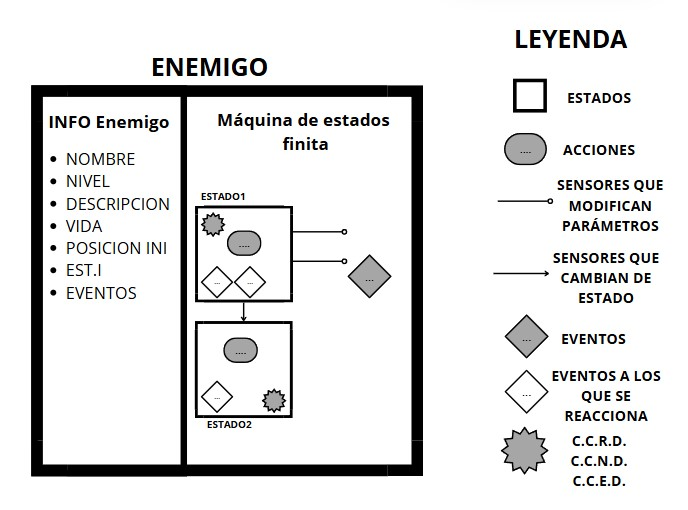
\includegraphics[height=5cm]{Imagenes/EnemigoGeneral.png}
	\caption{Enemigo General }
	\label{fig:EnemigoGeneral}
\end{figure}
Estos conceptos (\hyperref[subsec:estado]{estados}, \hyperref[subsec:acciones]{acciones}, \hyperref[subsec:sensores y emisores]{sensores y emisores}) se desarrollan con mayor detalle en los apartados siguientes.

\section{Ejemplos de uso}
Con esta separación de actuadores, sensores y daño la creación de enemigos se vuelve mucho más sencilla. A continuación se presentan unos ejemplos construidos mediante la combinación de los componentes de la herramienta sin la necesidad de escribir código.

\subsection{Enemigo patrullero}
Descripción:  El enemigo se desplaza de izquierda a derecha hasta colisionar, momento en el que invierte su dirección. Este patrón básico es común en enemigos de bajo nivel o como obstáculos simples. \\
Movimiento: Horizontal

\subsection{ Perseguidor aéreo con movimiento circular}
Descripción: Enemigo volador que se mueve describiendo un círculo alrededor de un punto mientras detecta la presencia del jugador. Puede emplearse como obstáculo en salas cerradas, generando presión por su presencia continua.\\
Movimiento: Circular

\subsection{Tubería de ácido}
Descripción: El enemigo permanece en una posición estática, pero representa una amenaza al disparar constantemente, obligando al jugador a esquivarlo o destruirlo antes de pasar.\\
Spawner: Genera gotas cada 2 segundos, por ejemplo.

\subsection{ Gota de ácido}
Descripción: Entidad que aparece desde una posición fija y se desplaza hacia abajo (simulando caída).

Movimiento: Vertical

\subsection{Enemigo con trayectoria}
Descripción: Enemigo que sigue una trayectoria ignorando al jugador. Por ejemplo andando alrededor de una plataforma\\
Movimiento: Spline Follower

\subsection{Cazador con persecución directa}
Descripción: Enemigo que detecta al jugador y se lanza directamente hacia él.
Dos estados:\\
Estado 1: 
Sensor: Distancia\\
Estado2:
Movimiento: Move To An Object 

